\subsection{Game Explorer}

\begin{figure}[h]
	\centering
	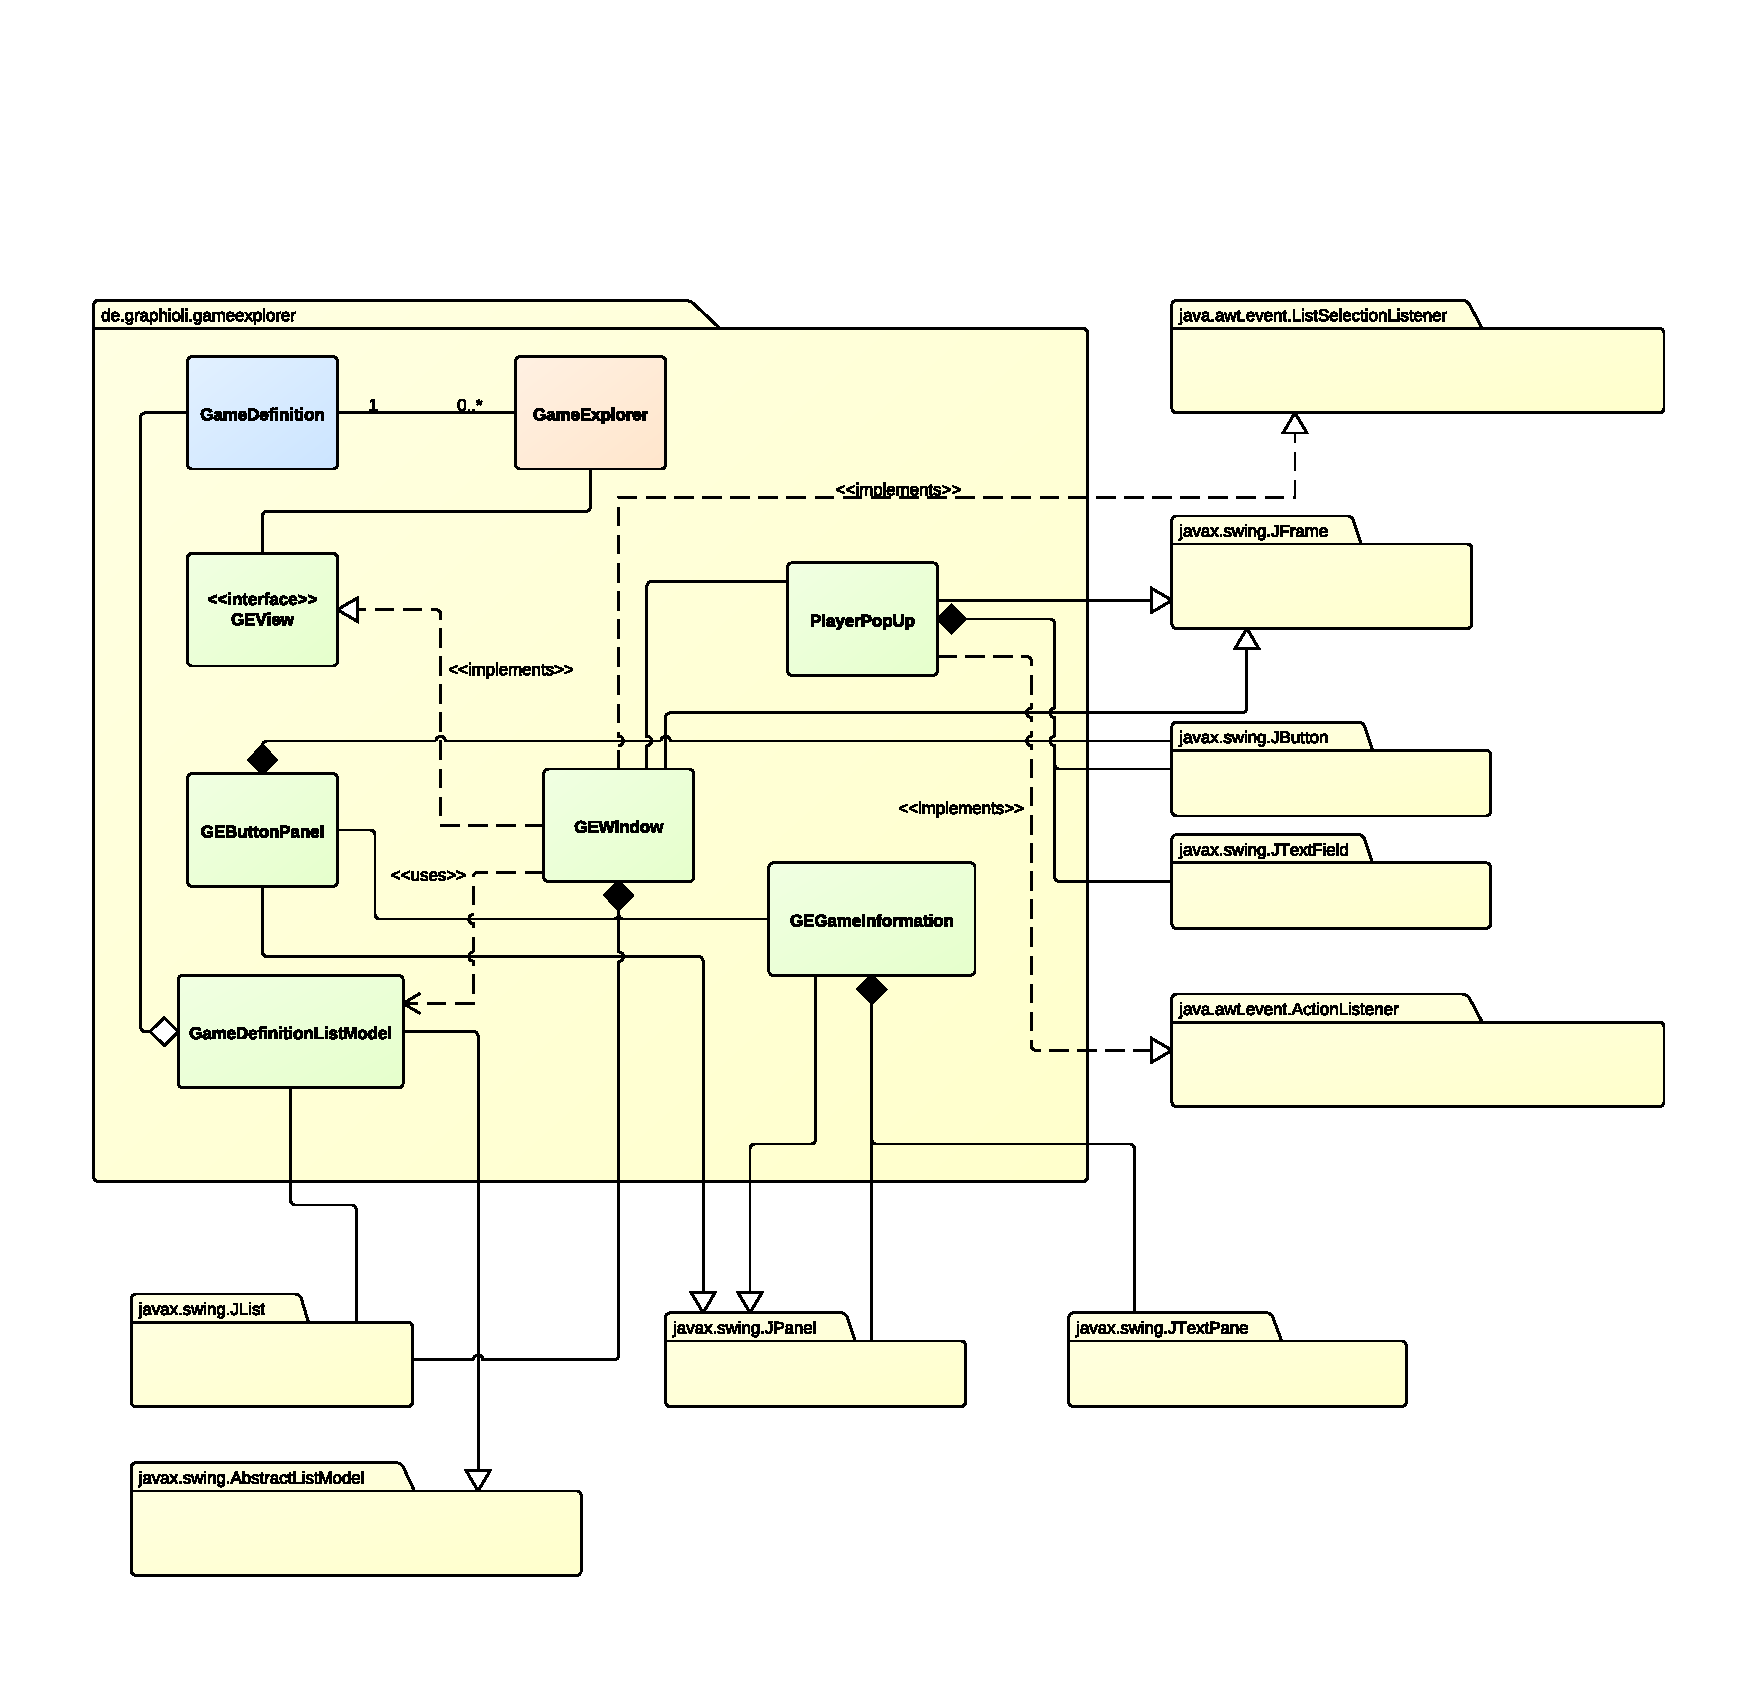
\includegraphics[page=1,width=\textwidth,keepaspectratio]{gameExplorerClassDiagram.pdf}
	\caption{GameExplorer class diagram.}
	\label{img:gameExplorerClassDiagram}
\end{figure}
\pagebreak

\class{GameExplorer}{gameexplorer}
\todo{Description} \\

\centerdash

\paragraph*{Method Summary}
\paragraph*{}
\begin{longtable}{Lp{10cm}}
	\startmethodtable
	\method{public}{GameExplorer(GameManager gameManager)}{ge:gameexplorer} \\
	& Creates a new \texttt{Game Explorer}. \\
	\method{private JSONObject}{parseJSON()}{ge:parsejson} \\
	& Parses the property file to a JSON Object. \\
	\method{private Iterable<GameDefinition>}{scanGameFolder()}{ge:scangamefolder} \\
	& Scans the \texttt{Game Folder} and returns the \ref{cls:gamedefinition}s of the games in it. \\
	\method{public boolean}{selectGame(GameDefinition gameDef)}{ge:selectgame} \\
	& description \\
	\method{public boolean}{openHelpFile(GameDefinition gameDef)}{ge:openhelpfile} \\
	& description \\
	\hline
\end{longtable}

\pagebreak

% GameDefinition
\class{GameDefinition}{gamedefinition}
This class represents the game's definition, containing crucial information that is needed to start a game.

\centerdash
\paragraph*{Method Summary}
\paragraph*{}
\begin{longtable}{Lp{10cm}}
	\startmethodtable
	\method{public}{GameDefinition({params})}{gd:gamedefinition} \\
	& Creates a new \texttt{GameDefinition} with the specified parameters. \\
	\method{public String}{getName()}{gd:getname} \\
	& Returns the \texttt{name} of this \texttt{GameDefinition}, which is the name of the game. \\
	\method{public int}{getMaxPlayerCount()}{gd:getmaxplayercount} \\
	& Returns the maximum number of players for this specific game. \\
	\method{public int}{getMinPlayerCount()}{gd:getminplayercount} \\
	& Returns the minimum number of players for this specific game. \\
	\method{public String}{getGamePath()}{gd:getgamepath} \\
	& Returns the path of this specific game. \\
	\method{public String}{getDescription()}{gd:getdescription} \\
	& Returns the description of this specific game. \\
	\method{public String}{getFullyQualifiedClassName()}{gd:getfullyqualifiedclassname} \\
	& Returns the fully qualified class name (e.g. ``de.graphioli.game.GraphColoring'') of this specific game. \\
	\method{public BufferedImage}{getScreenshot()}{gd:getscreenshot} \\
	& Returns a \texttt{BufferedImage} that is this game's screenshot. \\
	\method{public File}{getLocalizedString()}{gd:getlocalizedstring} \\
	& Returns a \texttt{String} telling which language file should be used. \\
	\method{public URI}{getHelpFile()}{gd:gethelpfile} \\
	& Returns the \texttt{URI} that links to the help file of this game. \\
	\method{public Iterable<MenuItem>}{getMenu()}{gd:getmenu} \\
	& Returns an iterable list of \texttt{MenuItem}s that will be used to generate this game's custom \texttt{MenuBar}. \\
	\method{public int}{getHorizontalGridPointCount()}{gd:gethorizontalgridpointcount} \\
	& Returns the number of horizontal \ref{cls:gridpoint}s for this specific game. \\
	\method{public int}{getVerticalGridPointCount()}{gd:getverticalgridpointcount} \\
	& Returns the number of vertical \ref{cls:gridpoint}s for this specific game. \\
	\hline
\end{longtable}

\pagebreak

\interface{GEView}{geview}
description \\

\centerdash

\paragraph*{Method Summary}
\paragraph*{}
\begin{longtable}{Lp{10cm}}
	\startmethodtable
	\method{public boolean}{registerController(GameExplorer gameExplorer)}{gev:registercontroller} \\
	& Registers the controller for the Game Explorer user interface. \\
	\hline
\end{longtable}

\pagebreak

\class{GEWindow}{gewindow}
This class represents the window of the \ref{cls:gameexplorer}. \\

\centerdash

\paragraph*{Method Summary}
\paragraph*{}
\begin{longtable}{Lp{10cm}}
	\startmethodtable
	\method{public}{GEWindow(Iterable<GameDefinition> games)}{gew:gewindow} \\
	& Creates a new \texttt{Game Explorer window}. \\
	\method{public}{onListSelectionChange(GameDefinition gameDef)}{gew:onlistselectionchange} \\
	& Updates the window when a game in the list is selected. \\
	\hline
\end{longtable}

\pagebreak

\class{GameDefinitionListModel}{gamedefinitionlistmodel}
Represents a data model that provides the \ref{cls:gegamelist} with its content. \\

\centerdash

\paragraph*{Method Summary}
\paragraph*{}
\begin{longtable}{Lp{10cm}}
	\startmethodtable
	\method{public}{GameDefinitionListModel(Iterable<GameDefinition> definitions)}{gdlm:gamedefinitionlistmodel} \\
	& Creates a new game definition list model with the given \ref{cls:gamedefinition}s. \\
	\method{public GameDefinition}{getGameDefinitionAtIndex(int index)}{gdlm:getgamedefinitionatindex} \\
	& Returns the \ref{cls:gamedefinition} at the given index. \\
	\hline
\end{longtable}

\pagebreak

\class{GEGameInformation}{gegameinformation}
Organizes the output of the screenshot and the description of the game \\

\centerdash

\paragraph*{Method Summary}
\paragraph*{}
\begin{longtable}{Lp{10cm}}
	\startmethodtable
	\method{public boolean}{setDescription(String description)}{gegi:setdescription} \\
	& Sets the description of the game and updates the display \\
	\method{public boolean}{setScreenshot(BufferedImage screenshot)}{gegi:setscreenshot} \\
	& Sets the screenshot of the game and updates the display \\
	\hline
\end{longtable}